% use paper, or submit
% use 11 pt (preferred), 12 pt, or 10 pt only

%\documentclass[letterpaper, preprint, paper,11pt]{AAS}	% for preprint proceedings
\documentclass[letterpaper, paper,11pt]{AAS}		% for final proceedings (20-page limit)
%\documentclass[letterpaper, paper,12pt]{AAS}		% for final proceedings (20-page limit)
%\documentclass[letterpaper, paper,10pt]{AAS}		% for final proceedings (20-page limit)
%\documentclass[letterpaper, submit]{AAS}			% to submit to JAS

\usepackage{bm}
\usepackage{amsmath}
\usepackage{subfigure}
%\usepackage[notref,notcite]{showkeys}  % use this to temporarily show labels
\usepackage[colorlinks=true, pdfstartview=FitV, linkcolor=black, citecolor= black, urlcolor= black]{hyperref}
\usepackage{overcite}
\usepackage{footnpag}			      	% make footnote symbols restart on each page
\usepackage[outdir=./]{epstopdf}

\PaperNumber{XX-XXX}

\begin{document}

\title{GPS Based Inertial Navigation For Low-Thrust Spacecraft In Cislunar Space}

\author{Grant R. Hecht\thanks{Graduate Student, Department of Mechanical and Aerospace Engineering, University at Buffalo, 240 Bell Hall, Buffalo, NY  14260-4400.}}

\maketitle{} 		

\begin{abstract}
	Missions to return to the Moon within the coming decade, which will involve manned and robotic spacecraft for extensive operations in lunar orbit and on the surface, require robust techniques for inertial navigation to ensure mission success. This paper investigates the feasibility of employing existing Earth based GPS navigation techniques for navigation in cislunar space. Both an Extended and Unscented Kalman Filter which employ GPS pseudorange and accelerometer measurements are developed and applied for inertial navigation of a low thrust spacecraft as it traverses from a geostationary transfer orbit to the target near-rectilinear halo orbit of the lunar gateway station, a key componant of NASA's Artemis Program. Through a Monte Carlo analysis, the performance of both developed filters are investigated and conclusions are drawn which point towards the overall feasibility of GPS based navigation for lunar missions, the best choice in filtering techniques, and methods which could improve the robustness of navigation in cislunar space. 
\end{abstract}

\section{Introduction}
Interest in manned and robotic missions to Earth's moon has been renewed with the advent of NASA's Artemis Program. As such, robust techniques for navigating spacecraft within cislunar space are necessary.  This project investigates the feasibility of employing pseudorange measurements from the existing GPS satellite constellation and IMU accelerometer measurements for navigating a low-thrust spacecraft as it spirals towards the target Near-Rectilinear Halo Orbit (NRHO) of the Artemis Lunar Gateway station, starting from a Geostationary Transfer Orbit (GTO) while employing both an Extended and Unscented Kalman Filter.

A feasibility study is performed to investigate the robustness of GPS based inertial navigation for a spacecraft traversing from a GTO to the NRHO target of the Gateway station. Both an Extended Kalman Filter (EKF) and Unscented Kalman Filter (UKF) have been developed which employ GPS pseudorange and accelerometer measurements for estimating the inertial states (e.g., position and velocity) and mass of a spacecraft as it travels from the initial to target orbits. The true GTO to NRHO trajectory has been generated for a low-thrust spacecraft by employing Circular Restricted Three-Body Problem (CR3BP) dynamics, such that fuel use is minimized. The performance of both the EKF and UKF are analyzed through Monte Carlo analysis.

The remainder of this paper is organized as follows. First, the methodology used throughout this investigation is discussed including the technique used for generating the true trajectory along with GPS pseudorange and accelerometer measurement modeling. Next, both inertial navigation filters (i.e., the EKF and UKF) are presented. Finally, the performance of both developed filters is investigated through Monte Carlo analysis and conclusions are drawn on the best choice of estimation algorithm for cislunar inertial navigation as well as additional sensors that could improve performance. 


\section{Methodology} 
\subsection{True Trajectory Generation}
The true low-thrust trajectory traversed by the spacecraft has been generated with CR3BP dynamics and a fully continuous, constant specific impulse thrust model by employing the \textit{indirect} approach to optimizing a spacecraft trajectory. Although many details of indirect optimal control are outside of the scope of this project, this category of trajectory optimization methods employ calculus of variations (COV) and Pontryagin's Maximum Principle (PMP) to analytically derive the necessary conditions of optimality. This process results in the formation of a two-point boundary value problem (TPBVP) which is solved by finding the set of time varying co-state (adjoint) variables at the initial epoch such that the boundary conditions are satisfied. 

For the minimum-fuel trajectory optimization problem, the cost function is given by
\begin{equation}
	J = \frac{T_{max}}{c}\int_{t_0}^{t_f}udt
\end{equation}
where $T_{max}$ is the maximum thrust available to the spacecraft, $c$ is the exhaust velocity, $u$ is the thrust throttling factor, and $t_i$ and $t_f$ correspond to the initial and final epoch of the trajectory. The TPBVP, while employing nondiamentionalized CR3BP dynamics, is formulated such that we seek state and co-state trajectories that are a solution of
\begin{align}
	\Dot{\mathbf{y}} = \begin{bmatrix} \Dot{\mathbf{x}} \\ 
	\Dot{\boldsymbol{\lambda}} \end{bmatrix} = \begin{bmatrix} \mathbf{v} \\ 
	\mathbf{g}(\mathbf{r}) + \mathbf{h}(\mathbf{v}) - \boldsymbol{\lambda}_vuT_{max}/(\lambda_vm) \\ 
	-uT_{max}/c \\ 
	-\mathbf{G}^T\boldsymbol{\lambda}_v \\ 
	-\boldsymbol{\lambda}_r - \mathbf{H}^T\boldsymbol{\lambda}_v \\ 
	-\lambda_vuT_{max}/m^2
	\end{bmatrix}
	\label{eqn:full_ode}
\end{align}
while satisfying 
\begin{equation}
	\begin{array}{ccc}
		\mathbf{r}(t_i) - \mathbf{r}_i = 0 & \mathbf{v}(t_i) - \mathbf{v}_i = 0 & m(t_i) - 1 = 0 \\
		\mathbf{r}(t_f) - \mathbf{r}_f = 0 & \mathbf{v}(t_f) - \mathbf{v}_f = 0 & \lambda_m(t_f) = 0 
	\end{array}
\label{eqn:state_cons}
\end{equation}
with optimal thrust direction unit vector and throttling factor given by Lawden's primer vector control law \cite{Lawden_1964, Hecht_2021, Russell_2007}, where $\mathbf{x} = [\mathbf{r},\mathbf{v},m]^T$ is the $7\times1$ vector of the position, velociy, and mass states, $\boldsymbol{\lambda}=[\boldsymbol{\lambda}_r,\boldsymbol{\lambda_v},\lambda_m]^T$ is the $7\times1$ vector of introduced co-state variables, corresponding to each of the physical states,
\begin{equation}
	\mathbf{g}(\mathbf{r}) = \begin{bmatrix}
	r_x - \frac{(1 - \mu)(r_x + \mu)}{r_1^3} - \frac{\mu(r_x + \mu - 1)}{r_2^3} \\
	r_y - \frac{(1 - \mu)r_y}{r_1^3} - \frac{\mu r_y}{r_2^3} \\
	-\frac{(1 - \mu)r_z}{r_1^3} - \frac{\mu r_z}{r_2^3}
	\end{bmatrix}
\end{equation}
\begin{equation}
	\mathbf{h}(\mathbf{v}) = \begin{bmatrix} 2v_y & -2v_x & 0 \end{bmatrix}^T
\end{equation}
\begin{align}
	r_1 &= \sqrt{(r_x + \mu)^2 + r_y^2 + r_z^2} \\
	r_2 &= \sqrt{(r_x + \mu - 1)^2 + r_y^2 + r_z^2}
\end{align}
and
\begin{align}
	\mathbf{G} &= \frac{\partial \mathbf{g}(\mathbf{r})}{\partial \mathbf{r}} \\
	\mathbf{H} &= \frac{\partial \mathbf{h}(\mathbf{v})}{\partial \mathbf{v}}
\end{align} 

The primary difficulty in solving this TPBVP involves determining an initial guess for the co-state variable such that convergence with a Newton's Method based solver can be achieved. For this work, Particle Swarm Optimization (PSO) was used to find multiple candidate trajectories (each corresponding to a local minimum of the minimum fuel cost function) for a fixed time of flight of 15 days as described in Reference \citenum{Hecht_2021} using spacecraft parameters shown in Table \ref{tab:traj_params}. Then, the TPBVP was resolved repeatedly for each of the candidate trajectories while gradually altering the time of flight in the direction of decreasing fuel use until the optimal time of flight for each of the candidate trajectories was discovered. Finally, of the improved candidate trajectories, the most fuel optimal solution was chosen, which was found to use 127 kg of fuel over 33 days. Figure \ref{fig:traj} displays this trajectory, where coasting arcs are shown in blue, thrusting arcs in red, the target NRHO in dashed black lines, and the locations of the Earth and Moon as black $\times$ symbols. As can be seen, the trajectory consists of multiple spirals about the Earth with gradually increasing apogee before finally reaching the NRHO. Therefore, this trajectory will provide a good indication of the developed filters performance in both near Earth and cislunar space.  

\begin{table}[]
	\centering
	\caption{Low-Thrust Trajectory Parameters}
	\label{tab:traj_params}
	\begin{tabular}{ccc}
		\hline
		\hline
		Parameter             		 & Value        & Units         \\ 
		\hline
		Initial Mass ($m_0$) 		 & 1500 		& kg            \\
		Exhaust Velocity (c) 		 & 29.43        & km/$\text{s}$  \\
		Specific Impulse ($I_{sp}$)  & 3000  		& s             \\
		Max Thrust ($T_{max}$)       & 10  		 	& N             \\
		%Time of Flight ($t_f-t_0$)   & 33.0      	& days          \\
		\hline \hline
	\end{tabular}
\end{table}

\begin{figure}[]
	\centering
	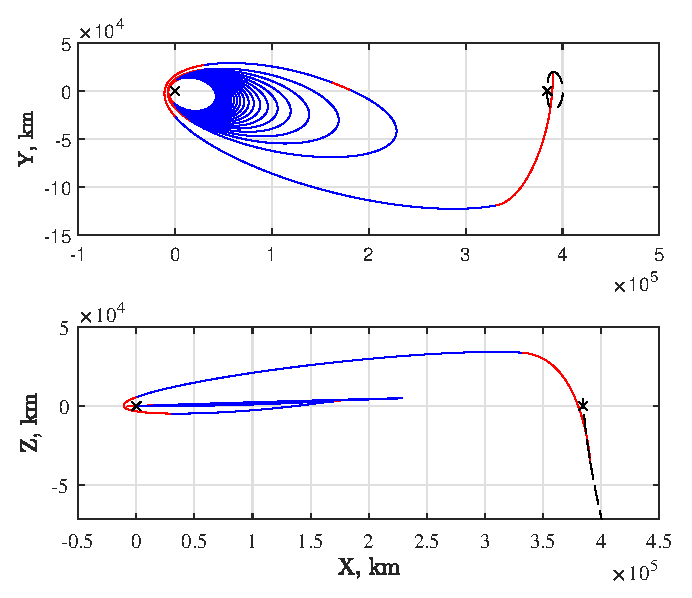
\includegraphics[width=0.75\textwidth]{./../../figures/iTraj.eps}
	\caption{True Low-Thrust Trajectory in Inertial Reference Frame}
	\label{fig:traj}
\end{figure}

Finally, whereas the true trajectory was generated using nondiamentionalized CR3BP dynamics which employ a rotating reference frame, we require the trajectory to be defined with respect to an inertial reference frame with dimensional units when using it to evaluate the performance of the developed inertial navigation filters. Therefore, the trajectories position, velocity, and mass states are dimentionalized using the time, length, velocity, and mass units given in Table \ref{tab:const_params} before rotation to the inertial frame according to 
\begin{align}
	\mathbf{r}^i &= \mathbf{T}_{sy}^i\mathbf{r}^{sy}  \\
	\mathbf{v}^i &= \mathbf{T}_{sy}^i\mathbf{v}^{sy} + \dot{\mathbf{T}}_{sy}^i\mathbf{r}^{sy}
\end{align}
where superscripts $sy$ and $i$ are used to denote a vector defined with respect to the synodic (rotating) and inertial reference frames respectively and
\begin{align}
	\mathbf{T}_{sy}^i &= \begin{bmatrix}
		\cos{\theta} & -sin(\theta) & 0 \\
		\sin{\theta} & \cos{\theta} & 0 \\
		0 & 0 & 1
	\end{bmatrix} \\
	\dot{\mathbf{T}}_{sy}^i &= \begin{bmatrix}
		-\omega\sin{\theta} & -\omega\cos{\theta} & 0 \\
		\omega\cos{\theta} & -\omega\sin{\theta} & 0 \\
		0 & 0 & 0
	\end{bmatrix}
\end{align}
where $\theta$ and $\omega$ are the angular rotation and rotational rate of the synodic reference frame with respect to the inertial frame respectively, where we select $\theta$ such that the Moon is aligned along the $y$-axis of the Inertial frame at the final epoch of the true trajectory.

\begin{table}[]
	\centering
	\caption{CR3BP Units}
	\label{tab:const_params}
	\begin{tabular}{ccc}
		\hline
		\hline
		Constant             & Value                     & Units           \\ 
		\hline
		Time Unit (TU)       & $3.75162997\times10^{5}$  & s               \\
		Length Unit (LU)     & $3.84400000\times10^{5}$  & km              \\
		Velocity Unit (VU)      & $1.02462131$              & km/s            \\
		Mass Unit (MU)       & $1500.0$                  & kg              \\
		\hline \hline
	\end{tabular}
\end{table}

\subsection{Measurement Modeling}\label{ssec:measmodeling}
\subsubsection{GPS Pseudoranges:}
A common GPS pseudorange model is given by \cite{Tapley_2004, Craft_2020}
\begin{align}
	p_{s,k} &= ||\boldsymbol{\rho}_{s/rk,k}|| + c(\Delta t_k - \Delta t_k^s) + \phi_k + v_{GPS,k} \\
	\boldsymbol{\rho}_{s/rk,k} &= \mathbf{r}_k^i + \mathbf{T}_b^i\mathbf{r}_{rx}^b - \mathbf{r}_{s,k}^i + \mathbf{T}_{b,s}^i\mathbf{r}_{pc,s}^b
\end{align}
where $p_{s,k}$ is the pseudorange generated from GPS satellite $s$ at time $t_k$, $\Delta t$ is the GNSS receiver clock bias, $\Delta t_k^s$ is the clock bias of GPS satellite $s$, $c$ is the speed of light in a vacuum, $\phi_{s,k}$ is the ionospheric delay, and $v_{GPS,k}$ is the receiver white noise. The geometric range is the Euclidean norm of the vector from the phase center of the GPS transmitter and GNSS receiver phase center $\boldsymbol{\rho}_{s/rk,k}$, where $\mathbf{r}_k^i$ is the inertial position of the satellite, $\mathbf{T}_b^i(\bar{\mathbf{q}}_{m,k}) \in SO(3)$ is the rotation from the body frame of the spacecraft to the inertial frame, $\mathbf{r}_{rx}^b$ is the location of the GNSS receiver phase center in the spacecrafts body frame, $\mathbf{r}_{s,k}^i$ is the inertial position of the center of mass of GPS satellite $s$, $\mathbf{T}_{b,s}^i\in SO(3)$ is the rotation from the body frame of GPS satellite $s$ to the inertial frame, and $\mathbf{r}_{pc,s}^b$ is the location of the phase center in the GPS body frame.

For the purposes of this work, we assume the phase centers of both the GNSS receiver and all GPS transmitters are located at their respective spacecraft's center of mass (i.e., $\mathbf{r}_{rx}^b = \mathbf{r}_{tx}^b = \mathbf{0}_{3\times1}$), thereby decoupling attitude from the pseudorange measurements. We will also assume the GNSS receiver clock is perfect, such that $\Delta t = 0$, and ionospheric effects are negligible. Therefore, our GPS pseudorange model reduces to
\begin{align}
	p_{s,k} &= ||\mathbf{r}_k^i - \mathbf{r}_{s,k}^i|| - c\Delta t_k^s + v_{GPS,k}
\end{align}
with relevent partials required by the EKF given by
\begin{equation}
	\frac{\partial p_s}{\partial \mathbf{r}^i}\bigg|_{\mathbf{x}=\mathbf{x}^*} \approx \frac{\mathbf{r}_k^{i^T} - \mathbf{r}_{s,k}^{i^T}}{||\mathbf{r}_k^i - \mathbf{r}_{s,k}^i||}
	\label{eqn:ppart}
\end{equation}
where $(\cdot)^*_k$ is employed to indicated a term associated with the reference trajectory at time $t_k$. Also, note that this partial is an approximation as we choose to neglect the effect of deviations in the position vector $\mathbf{r}_k^i$ on signal transmission time and therefore $\mathbf{r}_{s,k}^i$.

High precision ephemeris data projects provided by IGS \cite{IGSproducts} are considered as truth and employed to compute the position of GPS satellites at signal transmission times when generating simulated GPS pseudorange measurements. Perturbed trajectory solutions from the same ephemerides are also employed when computing expected pseudorange measurements so as to simulate much less precise broadcast ephemeris. 

When simulating GPS pseudorange measurements or computing expected measurements within both of the investigated filters, it is important to take into account signal transmission delay. While we choose to ignore atmospheric effects on the rate of signal transmission for simplicity, the velocity of signal propagation through the vacuum of space is still capped at the speed limit of the universe, i.e., the speed of light ($c=299792458$ m/s). Therefore, the time of signal transmission and reception will differ slightly and given the time of signal reception, $t_k$, the transmission time from satellite $s$, $t_{tx,s}$, can be found by determining the zero of the nonlinear equation given by 
\begin{equation}
	f(t_{tx,s}) = ||\mathbf{r}_k^i - \mathbf{r}_{s,k}^i|| - c(t_k - t_{tx,s})
\end{equation}

It is also important to note that IGS ephemeris data products are defined with respect to the Earth fixed IGS14 reference frame, and therefore must be rotated to the Geocentric Celestial Reference Frame (e.g., J200 frame) before they can be employed for inertial navigation. We perform this rotation with high precision by taking into account the Earth's polar motion, rotation, precession, and nutation as described by Vallado in Reference \citenum{Vallado_2013}.

\subsubsection{Inertial Measurement Unit}
IMU accelerometer measurements can be modeled as 
\begin{equation}
	\mathbf{a}_{m,k}^{IMU} = (\mathbf{I} + \mathbf{N}_a + \mathbf{M}_a)(\mathbf{I} + \mathbf{S}_a)(\mathbf{a}_k^{IMU} + \mathbf{b}_{a,0} + \mathbf{b}_{a,k} + \mathbf{v}_{a,k})
\end{equation}
where $\mathbf{a}_k^{IMU}$ is the true acceleration experienced by the IMU within the IMU frame, $\mathbf{b}_{a,0}$ is the startup bias of the accelerometer, $\mathbf{b}_{a,k}$ is the bias of the accelerometer at $t_k$, $\mathbf{v}_k$ is zero-mean white noise, $\mathbf{S}_a$ is the scale factor error matrix, $\mathbf{M}_a$ is the axes misalignment matrix, and $\mathbf{N}_a$ is the axes nonorthogonality matrix \cite{DeMars_2014}.

For the purposes of this investigation, we choose to simplify this model significantly, assuming most sources of error are negligible such that the measured acceleration in the IMU frame is given by 
\begin{align}
	\mathbf{a}_{m,k}^{IMU} = \mathbf{a}_k^{IMU} + \mathbf{v}_{a,k}
\end{align}
We will also assume the spacecraft body frame and IMU frame are always perfectly aligned with the inertial frame (i.e., $\mathbf{a}_{m,k}^{IMU}=\mathbf{a}_{m,k}^i$), thereby allowing the attitude of the spacecraft to be ignored as attitude estimation is outside of the scope of this work. 

The relevant partials of the accelerometer measurements for the EKF, assuming perfectly spherical gravitational effects from both the Earth and Moon, are then given by
\begin{align}
	\frac{\partial \mathbf{a}_{m}^i}{\partial \mathbf{r}^i}\bigg|_{\mathbf{x}=\mathbf{x}^*} &= \frac{\mu}{r^3}\left(\frac{3}{r^2}\mathbf{r}^i\mathbf{r}^{i,T} - \mathbf{I}\right) + \frac{\mu_l}{r_{ls}^3}\left(\frac{3}{r_{ls}^2}\mathbf{r}_{ls}^i\mathbf{r}_{ls}^{i,T} - \mathbf{I}\right) \label{eqn:apartr}\\
	\frac{\partial \mathbf{a}_{m}^i}{\partial m}\bigg|_{\mathbf{x}=\mathbf{x}^*} &= -\frac{u T_{max}}{m^2}\boldsymbol{\alpha}^i
	\label{eqn:apartm}
\end{align}
where $\mathbf{r}_{ls}^i$ is the vector from the spacecraft to the Moon defined with respect to the inertial reference frame, $r$ and $r_{ls}$ are the Euclidean norm of $\mathbf{r}^i$ and $\mathbf{r}_{ls}^i$ respectively, $\mu$ and $\mu_l$ are the gravitational parameters of the Earth and Moon respectively, $T_{max}$ is the spacecrafts maximum possible thrust, $u$ is the thrust throttling factor, and $\boldsymbol{\alpha}^i$ is the direction of applied propulsive force.

\section{Inertial Navigation Filters}
For the development of both the EKF and UKF, we begin with the nonlinear dynamics and measurement models given by \cite{Crassidis_2004}
\begin{align}
	\dot{\mathbf{x}}(t) &= \mathbf{f}(\mathbf{x}(t), \mathbf{u}(t),t) + \mathbf{G}(t)\mathbf{w}(t), \hspace{2mm} \mathbf{w}(t)\sim N(\mathbf{0},\mathbf{Q}(t)) \\
	\tilde{\mathbf{y}}_k &= \mathbf{h}(\mathbf{x}_k) + \mathbf{v}_k, \hspace{2mm} \mathbf{v}_k \sim N(\mathbf{0}, \mathbf{R}_k) 
\end{align}
where $\mathbf{x}(t)$ is the state-to-be-estimated, defined as the concatenation of the inertial position and velocity vectors and the mass of the spacecraft, $\mathbf{u}(t)$ is the control applied by the spacecraft, which consists of the throttling factor $u$ and thrust direction $\boldsymbol{\alpha}^i$ that are assumed to be known perfectly, $\mathbf{w}$ is defined as the process noise which accounts for imperfectly modeled dynamics, assumed to be a zero mean Gaussian random variable with covariance $\mathbf{Q}(t)$. Also, $\mathbf{h}(\mathbf{x}_k)$ is the measurement taken at time $t_k$, which can include only the three accelerometer measurement, only $l\in[0,32]$ pseudorange measurements from the $l$ visible GPS satellites, or a combination of both accelerometer and GPS pseudorange measurements, and $\mathbf{R}_k$ is the measurement covariance matrix. Furthermore, $\mathbf{f}(\mathbf{x}(t), \mathbf{u}(t), t)$ is the dynamics which are given by
\begin{equation}
	\mathbf{f}(\mathbf{x}(t),\mathbf{u}(t),t) = \begin{bmatrix} 
		\mathbf{v}^i \\ 
		-\frac{\mu}{r^3}\mathbf{r}^i + \mu_l\left(\frac{\mathbf{r}_{ls}^i}{r_{ls}^3} - \frac{\mathbf{r}_l^i}{r_l^3}\right)  + \frac{uT_{max}}{m}\boldsymbol{\alpha}^i \\
		-uT_{max}/c
	\end{bmatrix}
\end{equation}
where we also assume ephemeris for the Moon is known perfectly and is used to compute $\mathbf{r}_{ls}^i$ and $\mathbf{r}_l^i$. 

\subsection{Extended Kalman Filter}
 \subsubsection{Propagation:}
The state estimate $\hat{\mathbf{x}}$ and error covariance matrix $\mathbf{P}$ are propagated within the EKF according to \cite{Crassidis_2004}
 \begin{align}
 	\dot{\hat{\mathbf{x}}} = \mathbf{f}(\hat{\mathbf{x}}(t), \mathbf{u}(t),t)
 \end{align}
\begin{equation}
	\dot{\mathbf{P}}(t) = \mathbf{F}(t)\mathbf{P}(t) + \mathbf{P}(t)\mathbf{F}^T(t) + \mathbf{G}(t)\mathbf{Q}(t)\mathbf{G}^T(t)
\end{equation}
where $\mathbf{G}$ is taken as the identity matrix, $\mathbf{F}$ is the dynamics Jacobian given by 
\begin{equation}
	\mathbf{F} = \frac{\partial \mathbf{f}}{\partial \mathbf{x}}\bigg|_{\hat{\mathbf{x}}(t),\mathbf{u}(t)} = \begin{bmatrix}
		\mathbf{0}_{3\times 3} & \mathbf{I}_{3\times3} & 0 \\
		\frac{\mu}{r^3}\left(\frac{3}{r^2}\mathbf{r}^i\mathbf{r}^{i,T} - \mathbf{I}\right) + \frac{\mu_l}{r_{ls}^3}\left(\frac{3}{r_{ls}^2}\mathbf{r}_{ls}^i\mathbf{r}_{ls}^{i,T} - \mathbf{I}\right)  & \mathbf{0} & -\frac{uT_{max}}{m^2}\mathbf{\alpha}^i \\
		\mathbf{0}_{1\times 3} & \mathbf{0}_{1\times 3} & 0
	\end{bmatrix}
\end{equation}
and $\mathbf{Q}$ was chosen as 
\begin{equation}
	\mathbf{Q} = \operatorname{diag}\left(\begin{bmatrix}
		0.0 & 0.0 & 0.0 & 1\times10^{-12} & 1\times10^{-12} & 1\times10^{-12} & 1\times10^{-3}
	\end{bmatrix} \right)
\end{equation}
Furthermore, the state estimate and error covariance matrix differential equations were numerically integrated employing Verner's ``most efficient'' 7(8) Runge-Kutta method \cite{Verner_2010} provided by the \textit{DifferentialEquations.jl} \cite{Rackauckas_2017} package written within the Julia programming language \cite{Bezanson_2017}.

 \subsubsection{Measurement Update:}
 The state estimate and error covariance matrix are updated within the EKF when a set of measurements is ingested
 according to \cite{Crassidis_2004}
 \begin{align}
 	\hat{\mathbf{x}}_k^+ &= \hat{\mathbf{x}}_k^- + \mathbf{K}_k\left[\tilde{\mathbf{y}}_k - \mathbf{h}(\hat{\mathbf{x}})\right] \\
 	\mathbf{P}_k^+ &= \left[\mathbf{I} - \mathbf{K}_k \mathbf{H}_k(\hat{\mathbf{x}}_k)\right]\mathbf{P}_k^-
 \end{align} 
where
\begin{equation}
	\mathbf{K}_k = \mathbf{P}_k^-\mathbf{H}_k^T(\hat{\mathbf{x}}_k^-)\left[\mathbf{H}_k(\hat{\mathbf{x}}_k^-)\mathbf{P}_k^-\mathbf{H}_k^T(\hat{\mathbf{x}}) + \mathbf{R}_k\right]^{-1}
\end{equation}

At this point, it is important to note that the number of measurements processed, as well as the size of $\mathbf{H}_k$ and $\mathbf{R}_k$, at a given epoch $t_k$ will differ due to differing IMU and GNSS receiver sampling rates as well as changes in the number of visible GPS satellites. Therefore, we'll consider three different scenarios: only accelerometer measurements are processed, only pseudorange measurements are processed, and both accelerometer and pseudorange measurements. 

For the case of only accelerometer measurements, the measurement vector is given by
\begin{equation}
	\tilde{\mathbf{y}}_{k,a} = \mathbf{a}_{m,k}^-
\end{equation}
and the expected measurement is computed as 
\begin{equation}
	\mathbf{h}_{a}(\hat{\mathbf{x}}_k) = 	-\frac{\mu}{||\hat{\mathbf{r}}||^3}\hat{\mathbf{r}} + \mu_l\left(\frac{\mathbf{r}_l^i - \hat{\mathbf{r}}}{||\mathbf{r}_l^i - \hat{\mathbf{r}}||^3} - \frac{\mathbf{r}_l^i}{r_l^3}\right)  + \frac{uT_{max}}{m}\boldsymbol{\alpha}^i 
\end{equation}
with a measurement Jacobian given by
\begin{equation}
	\mathbf{H}_{a,k} = \frac{\partial \mathbf{h}_a}{\partial \mathbf{x}}\bigg|_{\hat{\mathbf{x}}_k,\mathbf{u}_k}  = \begin{bmatrix}
		\frac{\partial \mathbf{a}^i_m}{\partial \mathbf{r}^i} & \mathbf{0}_{3\times 3} & \frac{\partial \mathbf{a}_m^i}{\partial m}
	\end{bmatrix}
\end{equation}
with partials given in Eqs. \eqref{eqn:apartr} and \eqref{eqn:apartm}, and measurement noise covariance matrix 
\begin{equation}
	\mathbf{R}_a = \operatorname{diag}(\begin{bmatrix}
		\sigma_a^2 & \sigma_a^2 & \sigma_a^2 
	\end{bmatrix})
\end{equation}
where a value of $\sigma_a = 10^{-3}$ m/$\text{s}^2$ was chosen to represent an IMU of moderate quality.

For the case of only $l$ pseudorange measurements, where $l\in[0, 32]$, the measurement vector is given by
\begin{equation}
	\tilde{\mathbf{y}}_{k,p} = \begin{bmatrix}
		p_{s_1,k} & p_{s_2,k} & \dots & p_{s_l,k}
	\end{bmatrix}^T
\end{equation} 
where subscript $s_1$ is simply used to denote the GPS satellite corresponding the first pseudorange measurement in $\tilde{\mathbf{y}}$ and does not imply $s=1$ or satellite PG01 as defined within IGS data products. Also, the expected measurement $\mathbf{h}_p(\hat{\mathbf{x}})$ is computed as described in the above section and the measurement Jacobian is given by
\begin{equation}
	\mathbf{H}_{p,k} = \frac{\partial \mathbf{h}_p}{\partial \mathbf{x}} \bigg|_{\hat{\mathbf{x}}_k,\mathbf{u}_k}  = \begin{bmatrix}
		\frac{\partial p_{s_1,k}}{\partial \mathbf{r}^i} & \mathbf{0}_{4\times 1} \\
		\frac{\partial p_{s_2,k}}{\partial \mathbf{r}^i} & \mathbf{0}_{4\times 1} \\
		\vdots & \vdots \\
		\frac{\partial p_{s_l,k}}{\partial \mathbf{r}^i} & \mathbf{0}_{4\times 1} 
	\end{bmatrix}
\end{equation}
Finally, the measurement covariance matrix is given by
\begin{equation}
	\mathbf{R}_p = \operatorname{diag}(\begin{bmatrix}
		\sigma_p^2 & \sigma_p^2 & \dots & \sigma_p^2
	\end{bmatrix})
\end{equation}
where a value of $\sigma_p = 10^{-2}$ km.

Finally, for the case of both pseudorange and accelerometer measurements, the measurement vector is given by
\begin{equation}
	\tilde{\mathbf{y}}_k = \begin{bmatrix}
		\tilde{\mathbf{y}}_{k,p} & \tilde{\mathbf{y}}_{k,a}
	\end{bmatrix}^T
\end{equation}
with expected measurements computed as
\begin{equation}
	\mathbf{h}(\hat{\mathbf{x}}_k) = \begin{bmatrix}
		\mathbf{h}_p(\hat{\mathbf{x}}_k) & \mathbf{h}_a(\hat{\mathbf{x}}_k)
	\end{bmatrix}^T
\end{equation}
and measurement Jacobian given by 
\begin{equation}
	\mathbf{H}_k = \frac{\partial \mathbf{h}}{\partial \mathbf{x}}\bigg|_{\hat{\mathbf{x}}_k,\mathbf{u}_k} = \begin{bmatrix}
		\mathbf{H}_{p,k} & \mathbf{H}_{a,k}
	\end{bmatrix}
\end{equation}
with a measurement covariance matrix
\begin{equation}
	\mathbf{R}_k = \begin{bmatrix}
		\mathbf{R}_p & \mathbf{0}_{l\times3} \\
		\mathbf{0}_{3\times l} & \mathbf{R}_a
	\end{bmatrix}
\end{equation}

\subsection{Unscented Kalman Filter}
\subsubsection{Propagation:}
The state estimate and error covariance matrix propagation step within the UKF first requires definition of the augmented covariance matrix given by 
\begin{equation}
	\mathbf{P}_k^a = \begin{bmatrix}
		\mathbf{P}_k^+ & \mathbf{0}_{7\times 7} \\
		\mathbf{0}_{7\times 7} & \mathbf{Q}_k
	\end{bmatrix}
\end{equation}
where we note that the measurement covariance matrix is not included to reduce the number of required sigma points and is instead added directly to the output covariance matrix to compute the innovations covariance (more on this in the following section) \cite{Crassidis_2004}. The propagation step begins with computation of the 29 sigma points as \cite{Crassidis_2004}
\begin{align}
	\boldsymbol{\chi}_k^{a(0)} &= \hat{\mathbf{x}}_k^a \\
	\boldsymbol{\chi}_k^{a(2i - 1)}  &=  \hat{\mathbf{x}}_k^a + \boldmath{\sigma}_k^i \hspace{1mm} \forall \hspace{1mm} i = 1,2,\dots,14 \\
	\boldsymbol{\chi}_k^{a(2i)}  &=  \hat{\mathbf{x}}_k^a - \boldmath{\sigma}_k^i \hspace{1mm} \forall \hspace{1mm} i = 1,2,\dots,14
\end{align}
where the augmented state vector is defined as \cite{Crassidis_2004}
\begin{align}
	\mathbf{x}_k^a = \begin{bmatrix}
		\mathbf{x}_k \\ \mathbf{w}_k
	\end{bmatrix}, \hspace{3mm} \hat{\mathbf{x}}_k^a = \begin{bmatrix}
		\hat{\mathbf{x}}_k \\ \mathbf{0}_{7\times 1}
\end{bmatrix}
\end{align}
and $\boldsymbol{\sigma}_k^i$ denotes the $i^{th}$ column of $\boldsymbol{\sigma}_k$ which is computed as
\begin{equation}
	\boldsymbol{\sigma}_k = \gamma \sqrt{\mathbf{P}_k^a}
\end{equation} 
with parameter $\gamma$ given by 
\begin{equation}
	\gamma = \sqrt{14 + \lambda}
\end{equation}
and 
\begin{equation}
	\lambda = \alpha^2(14 + \kappa) - 14
\end{equation}
where we've chosen $\alpha=1.0$ and $\kappa = 17.0$. Once the sigma points have been computed, each is propagated to $t_{k+1}$ by numerically integrating the differential equations
\begin{equation}
	\dot{\boldsymbol{\chi}}^{x(i)} = \mathbf{f}(\boldsymbol{\chi}^{x(i)}(t),\mathbf{u}(t), t)  + \boldsymbol{\chi}_k^{w(i)}\hspace{1mm}\forall\hspace{1mm}i=0,1,\dots,28
\end{equation}
where 
\begin{equation}
	\boldsymbol{\chi}_k^{a(i)} = \begin{bmatrix}
		\boldsymbol{\chi}_k^{x(i)} \\ \boldsymbol{\chi}_k^{w(i)}
	\end{bmatrix}
\end{equation}
for which we again employ Verner's 7(8) Runge-Kutta method. Then, the predicted state estimate and error covariance are computed as \cite{Crassidis_2004}
\begin{align}
	\hat{\mathbf{x}}_{k+1}^- &= \sum_{i=0}^{28}W_i^{\text{mean}}\boldsymbol{\chi}_{k+1}^{x(i)} \\
	\mathbf{P}_{k+1}^- &= \sum_{i=0}^{28}W_i^{\text{cov}} \left[\boldsymbol{\chi}_{k+1}^{x(i)} - \hat{\mathbf{x}}_{k+1}^-\right]\left[\boldsymbol{\chi}_{k+1}^{x(i)} - \hat{\mathbf{x}}_{k+1}^-\right]^T
\end{align}
with weights given by
\begin{align}
	W_0^\text{mean} &= \frac{\lambda}{14 + \lambda} \\
	W_0^\text{cov} &= \frac{\lambda}{14 + \lambda} + (1 - \alpha^2 + \beta) \\
	W_i^\text{mean} &= W_i^\text{cov} = \frac{1}{2(14 + \lambda)}
\end{align}
where $\beta = 0.0$ was selected. 

\subsection{Measurement Update:}
The state estimate and error covariance matrix are then updated within the UKF by ingesting a set of measurements $\tilde{\mathbf{y}}_k$ which vary in size as described above within the EKF section. This process begins with the computation of the mean observation as \cite{Crassidis_2004}
\begin{equation}
	\hat{\mathbf{y}}_k^- = \sum_{i=0}^{28}W_i^\text{mean} \boldsymbol{\gamma}_k^i
\end{equation}
where
\begin{equation}
	\boldsymbol{\gamma}_k^i = \mathbf{h}(\boldsymbol{\chi}_k^{x(i)}, \mathbf{u}_k,k)
\end{equation}
Then the output covariance is computed as 
\begin{equation}
	\mathbf{P}_k^{yy} = \sum_{i=0}^{28}W_i^\text{cov}\left[\boldsymbol{\gamma}_k^i-\hat{\mathbf{y}}_k^-\right]\left[\boldsymbol{\gamma}_k^i-\hat{\mathbf{y}}_k^-\right]^T
\end{equation}
which is used to compute the innovations covariance as
\begin{equation}
	\mathbf{P}_k^{e_ye_y}=\mathbf{P}_k^{yy} + \mathbf{R_k}
\end{equation}
where the measurement covariance matrix is defined as described above for the EKF. Finally, the cross-correlation matrix is computed as \cite{Crassidis_2004}
\begin{equation}
	\mathbf{P}_k^{e_xe_y} = \sum_{i=0}^{28}W_i^\text{cov}\left[\boldsymbol{\chi}_k^{x(i)}-\hat{\mathbf{x}}_k^-\right]\left[\boldsymbol{\gamma}_k^i - \hat{\mathbf{y}}_k^-\right]
\end{equation}
and the state and error covariance matrix are updated according to
\begin{align}
	\hat{\mathbf{x}}_k^+ &= \hat{\mathbf{x}}_k^- + \mathbf{K}_k\mathbf{e}_k^- \\
	\mathbf{P}_k^+ &= \mathbf{P}_k^- - \mathbf{K}_k\mathbf{P}_k^{e_ye_y}\mathbf{K}_k^T
\end{align}
where 
\begin{equation}
	\mathbf{e}_k^- = \tilde{\mathbf{y}}_k - \hat{\mathbf{y}}_k^-
\end{equation}
and
\begin{equation}
	\mathbf{K}_k = \mathbf{P}_k^{e_xe_y}\left(\mathbf{P}_k^{e_ye_y}\right)^{-1}
\end{equation}

\section{Results}
To investigate the performance of the developed filters as well as the feasibility of inertial navigation in cislunar space using the Earth orbiting GPS constellation, a Monte Carlo analysis was performed. Both filters were ran for 100 independent trials, each time sampling the initial state estimate according to
\begin{equation}
	\hat{\mathbf{x}}_0 = N(\mathbf{x}_0, \mathbf{P}_0^+)
\end{equation}
where $\mathbf{x}_0$ is the true initial state and $\mathbf{P}_0^+$ initial state estimate error covariance matrix chosen as
\begin{equation}
	\mathbf{P}_0^+ = \operatorname{diag}(\begin{bmatrix}
		\sigma_r^2 & \sigma_r^2 & \sigma_r^2  & 	\sigma_v^2 & \sigma_v^2 & \sigma_v^2 & \sigma_m^2
	\end{bmatrix})
\end{equation}
with $\sigma_r = 100 $ m, $\sigma_v=10.0$ m/s, and $\sigma_m=1.0$ mg. Also, both the accelerometer and pseudorange measurement noise standard deviation values given above were used, i.e., $\sigma_a = 10^{-3}$ m/$\text{s}^2$ and $\sigma_p=10.0$ m. Finally, to reduce memory requirements when saving data for the full 33 day trajectory, both the accelerometer and pseudorange measurements were taken at a lower frequency than would likely be done in practice. For the EKF, accelerometer measurements were processed every 30 seconds and pseudorange measurements every 15 minutes. Similarly, accelerometer measurements were processed every minute and pseudorange measurements again every 15 minutes for the UKF. It was decided to reduce the frequency of accelerometer measurements further for the UKF when compared to the EKF due to the decreased computational efficiency of the algorithm.

\subsection{EKF Results}

\begin{figure}
	\centering 
	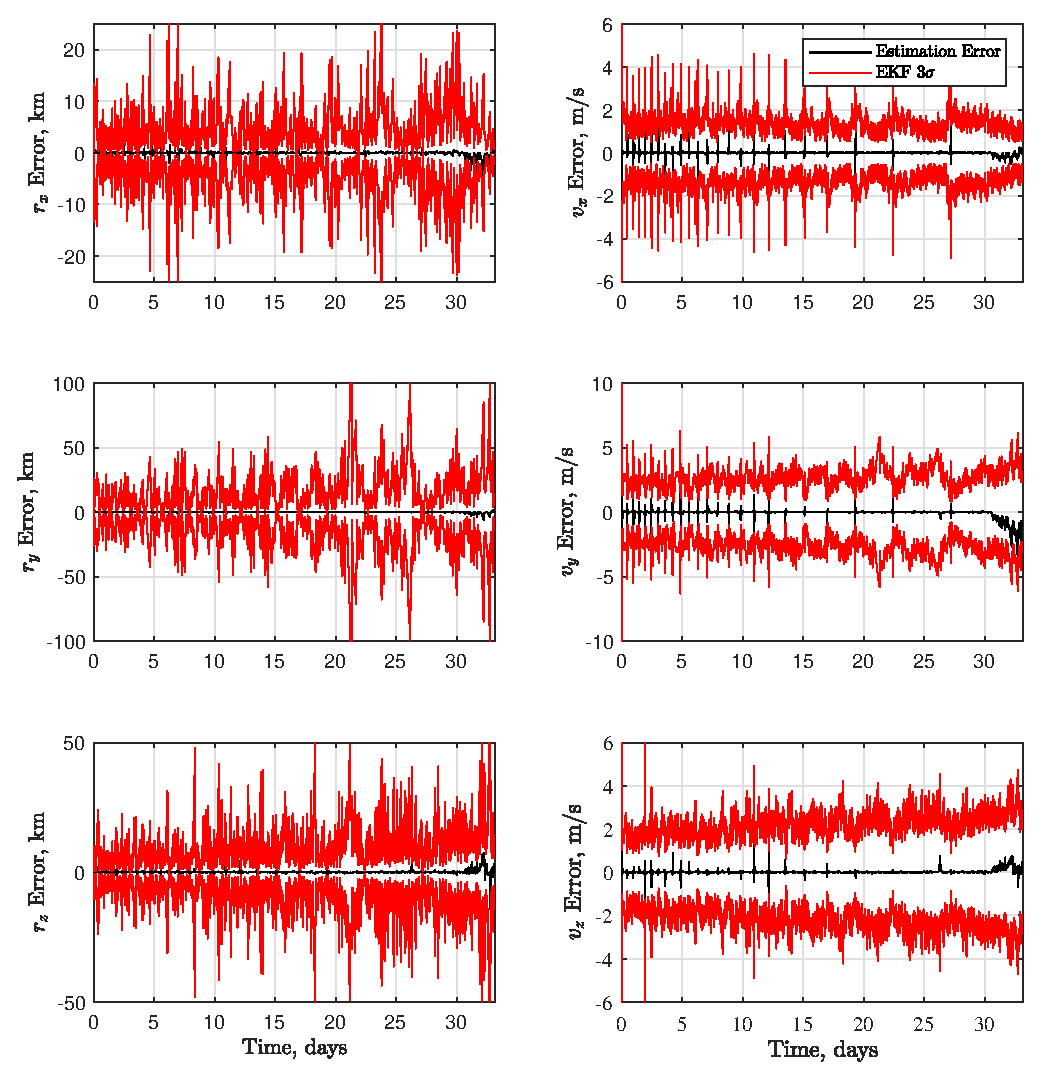
\includegraphics{./../../figures/EKFPosVelError.eps}
	\caption{EKF Inertial Estimation Error and Uncertainty}
	\label{fig:EKFposvelerr}
\end{figure}

\begin{figure}
	\centering 
	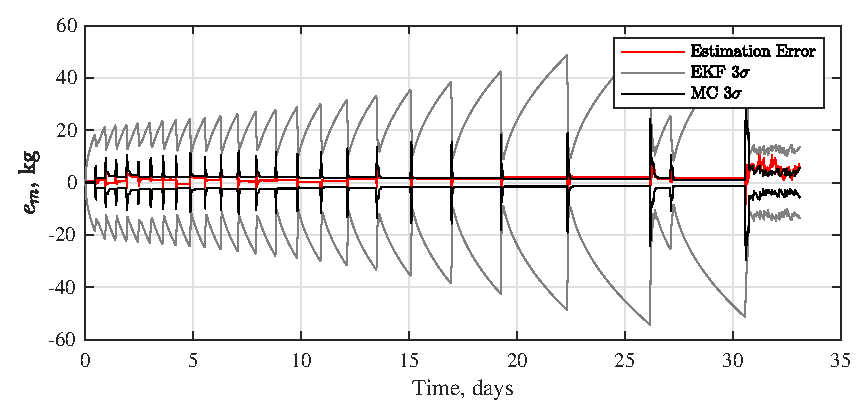
\includegraphics{./../../figures/EKFMassError.eps}
	\caption{EKF Mass Estimation Error and Uncertainty}
	\label{fig:EKFmasserr}
\end{figure}

Figures \ref{fig:EKFposvelerr} and \ref{fig:EKFmasserr} display the estimation error and the filters realization of its uncertainty as $3\sigma$ bounds from a single trial along with the Monte Carlo error $3\sigma$ bounds for the inertial states and mass respectively. 

Focusing first on the position error plots in Figure \ref{fig:EKFposvelerr}, we can see that the position estimation error in the three Cartesian directions of the inertial reference frame remains bounded by the filters $3\sigma$ bounds for a majority of the 33 day trajectory. Furthermore, we can see that when the position error does leave the $3\sigma$ bounds (see plots corresponding to the $x$- and $z$-axis after about $27$ days)  it quickly converges back within the bounds. Also, it's important to note that the error and $3\sigma$ bounds do begin to grow as the spacecraft nears the Moon (after around 30 days) and we can also see slight peaks in the $3\sigma$ bounds which correspond to the spacecraft reaching the apoapsis of it current spiral trajectory about the Earth, both of which make intuitive sense as the spacecraft is traveling further from the GPS constellation resulting in the system becoming less observable. Finally, when comparing the filters realization of its uncertainty with the Monte Carlo error statistics, we can see that while both maintain a similar trend, the EKF is overly modest and ``believes'' it's is worse than it actually is. It's important to note that this quality of the filter could likely be improved with further tuning of the process noise. Furthermore, 100 Monte Carlo trials is still relatively low (around 1000 would likely be more ideal) and it is therefore possible that the Monte Carlo statistics are not an accurate representation of the true error statistics.

Moving our focus to the velocity error plots of Figure \ref{fig:EKFposvelerr}, we again see a similar trend, with the error bounded by the filters $3\sigma$ bounds for a majority of the trajectory, again only leaving the bounds briefly after around 27 days. We also see the estimation error and uncertainty growing as the spacecraft approaches the Moon, as well as at each apoapsis of the trajectory, although the velocity estimation uncertainty appears to rapidly grow and shrink, manifesting as vertical spikes in the $3\sigma$ bounds which are especially visible in the plot corresponding to the x-direction. Finally, we can see the filters representation of its uncertainty to follow a similar trend with the Monte Carlo error statistics and is again modest, over representing its estimation uncertainty.

Shifting focus to Figure \ref{fig:EKFmasserr}, we again see the mass estimation error is bounded by the filters $3\sigma$ bounds, here for the entire duration of the trajectory.  Interestingly, we do again see repeated increases in the filters mass estimation uncertainty before rapidly decreasing with gradually decreasing frequency. This phenomena is not related to increasing distance from the GPS constellation though (as it was for both position and velocity estimation) and instead the rapid decrease in uncertainty corresponds to the moments at which the thruster is firing, as this is the only time the mass of the spacecraft is observable. Although not investigated in the work, this behavior could likely be improved by setting the process noise for the mass dynamics to zero when the thruster is not firing, as we know that mass will remain constant when fuel is not being used. We can also see that the mass estimation error remains nearly constant for increasingly longer duration with the same frequency as the spikes in uncertainty which is also directly related to the moments at with the thruster is not firing. Also, quite different from the inertial state estimation, we can see the filters uncertainty is at its lowest point when approaching the moon for the final 3 days of the journey which results from the long thrusting arc used to place the spacecraft on the NRHO. Finally, comparing the filters realization of its mass estimation uncertainty with the Monte Carlo statistics, we can see that both do not follow a similar trend due to the process noise included when the thruster is not firing. Furthermore, the Monte Carlo $3\sigma$ bounds also appear to under represent the mass estimation error, especially near the end of the trajectory. This is due to relatively large bias in the estimation of the spacecrafts mass, which we will further investigate in the following discussion. 

\begin{figure}
	\centering 
	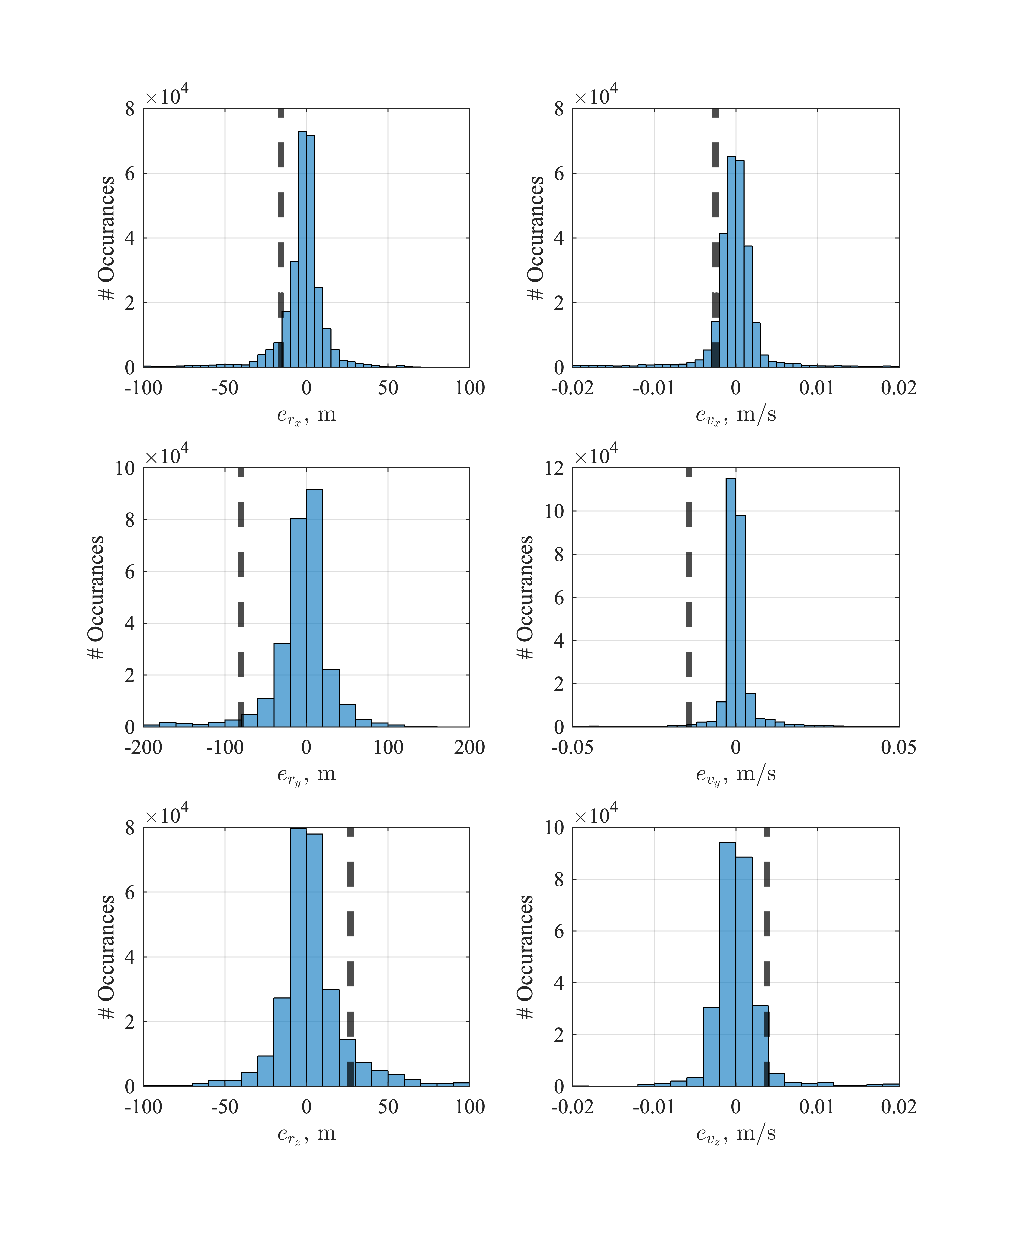
\includegraphics{./../../figures/EKFPosVelHist.eps}
	\caption{EKF Inertial State Estimation Error Distributions}
	\label{fig:EKFposvelhist}
\end{figure}

\begin{figure}
	\centering 
	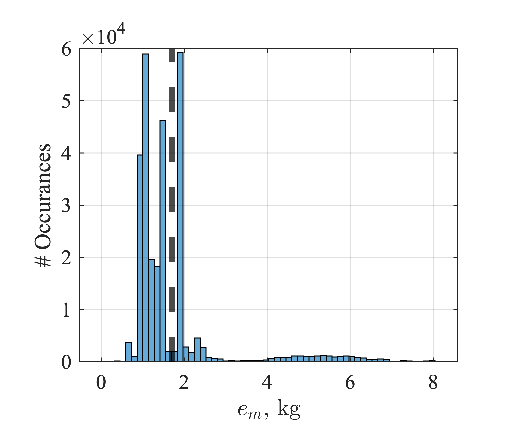
\includegraphics{./../../figures/EKFMassHist.eps}
	\caption{EKF Mass Estimation Error Distribution}
	\label{fig:EKFmasshist}
\end{figure}

To further investigate the distribution of the estimation errors, as well as to shed light on any bias present, Figures \ref{fig:EKFposvelhist} and \ref{fig:EKFmasshist} display histograms of the inertial states and mass respectively from each trial of the Monte Carlo analysis along with a vertical dashed line corresponding the mean of each distribution. When viewing these figures, it's important to note that the mean does not look correct which is due to many outliers of each distribution falling outside of the limits of the x-axis of each figure.

Focusing first on the distributions of the inertial state estimation errors shown in Figure \ref{fig:EKFposvelhist}, we can see that a large majority of the errors appear to be distributed normally with zero mean in all cases. With that said, each distribution also contains many outliers which result in a mean that is shifted away from zero. Although not shown in each plot, these outliers did not appear to congregate about a second mode (i.e., the distributions did not appear to be multi-modal) and therefore would not be visible due to the large magnitude of occurrences centered about zero. Although these plots do appear to show bias in the estimation of each state, it is possible that this behavior would disappear with more more Monte Carlo trials. Also, while examining these plots we can see the estimation accuracy in much more detail when compared to Figure \ref{fig:EKFposvelerr}. Clearly the EKF did quite well, often estimating the position along the $x$- and $z$-directions within 100 m and in the $y$-direction within 200 m. Furthermore, estimation of the velocity was even better, with the EKF determining the velocity in each of the Cartesian direction to within 50 mm/s in a majority of cases. 

Shifting focus to Figure \ref{fig:EKFmasshist}, we see an entirely different trend with the distribution of mass estimation errors when compared to those shown in Figure \ref{fig:EKFmasshist}. From this plot, we can observe a clear bias and a distribution that appears to be multi-modal, with two modes centered around 2 kg and a third centered about 5.5 kg. It is theorized that this behavior is due to the nonlinearity of the orbital dynamics, as well as the poor observability of the mass. Not only is the mass only observable when the spacecraft is thrusting, but the magnitude of the thrust is also quite small at only 10 N resulting in an acceleration due to thrust that is much lower in magnitude than the gravitational acceleration, especially when near the Earth where a majority of the thrusting occurs, which produces further difficulty.  Despite the clear bias and poor observability, the EKF does still estimate the mass of the spacecraft with surprising accuracy with a maximum mass estimation error of only 8.1 kg out of all 100 trials. 

\subsection{UKF Results}
\begin{figure}
	\centering 
	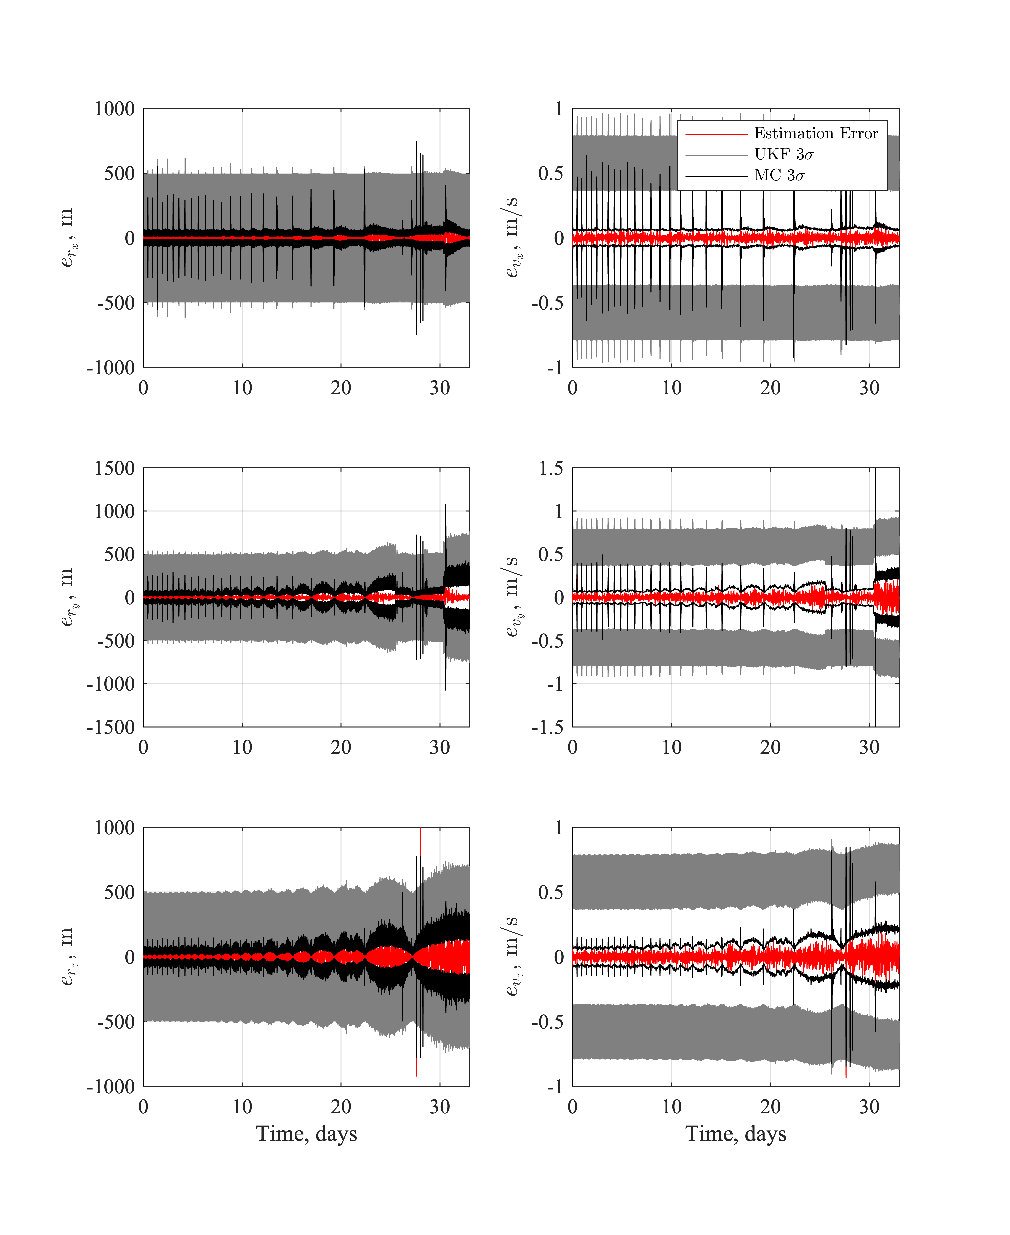
\includegraphics{./../../figures/UKFPosVelError.eps}
	\caption{UKF Inertial Estimation Error and Uncertainty}
	\label{fig:UKFposvelerr}
\end{figure}

\begin{figure}
	\centering 
	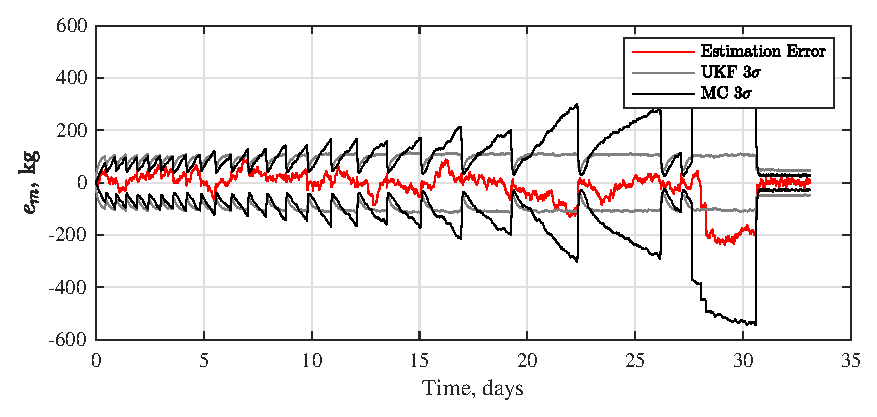
\includegraphics{./../../figures/UKFMassError.eps}
	\caption{UKF Mass Estimation Error and Uncertainty}
	\label{fig:UKFmasserr}
\end{figure}

Moving our discussion to results obtain using the UKF, Figures \ref{fig:UKFposvelerr} and \ref{fig:UKFmasserr} display the estimation error and the filters realization of its uncertainty as $3\sigma$ bounds from a single trial along with the Monte Carlo error $3\sigma$ bounds for the inertial states and mass respectively. 

Focusing first on the position error plots in Figure \ref{fig:UKFposvelerr}, we can see that the position estimation error in the three Cartesian directions of the inertial reference frame again remain bounded by the filters $3\sigma$ bounds for a majority of the trajectory. Furthermore, for the single trial shown, the error only leaves the $3\sigma$ bounds twice, both with the estimates of the position in the $z$-direction at around 28 days and quickly converges back within the bounds. Also, we see a similar trend observed with the EKF, that being the uncertainty grows about the apoapsis of each spiral until ballooning out to its largest point when approaching the Moon. With that said, this trend is less visible in the UKF's realization of its uncertainty when compared to the EKF, especially before the 15 day mark, but we can see it with much more clarity when looking at the Monte Carlo $3\sigma$ bounds. One significant trend observed here but not for the EKF is the ``jittering'' or rapid oscillation in the filters $3\sigma$ bounds, resulting in the UKF's $3\sigma$ bounds appearing as a thick band in Figure \ref{fig:UKFposvelerr}. This phenomena occurred due to the correction when ingesting GPS pseudorange measurements exhibiting a much more profound improvement on the quality of the state estimate when compared to the EKF. Finally, when comparing the filters uncertainty with the Monte Carlo $3\sigma$ bounds, we can see that both follow nearly the exact trend, with each peek and trough of the two bounds matching up nearly one-to-one which clearly demonstration the UKF's improved ability in representing it's uncertainty as compared to the EKF. With that said, the UKF is also modest, although not as much as the EKF, but this could very likely be improved with further tuning of the process noise and $\alpha$, $\beta$, and $\kappa$ parameters. 

Moving our focus to the velocity error plots of Figure \ref{fig:UKFposvelerr}, we once again see a similar trend, with the error bounded by the filters $3\sigma$ bounds for the entire trajectory. We also see the estimation error and uncertainty growing as the spacecraft approaches the Moon, as well as at each apoapsis of the trajectory as we've noted for estimation of all inertial states of the spacecraft, both with the EKF and UKF. Furthermore, we again see the same vertical spikes observed with the EKF in the filters $3\sigma$ bounds corresponding to the velocity in the $x$-direction. The jittering in the UKF's $3\sigma$ bounds is also again present when estimating the velocity of the spacecraft. Finally, we can see the filters representation of its uncertainty follows the trend exhibited by the Monte Carlo $3\sigma$ bounds nearly exactly as was also noted for the position states, although the filter is clearly modest in this case with the filters $3\sigma$ bounds separated from the Monte Carlo bounds by about 0.4 m/s in all cases. 

Shifting focus to Figure \ref{fig:UKFmasserr}, we see that the UKF actually performs much worse for a majority of the trajectory when estimating the mass of the spacecraft when compared to the EKF, with the mass estimation error leaving the filters $3\sigma$ bounds for a significant duration around day 27 to 31. It is expected that a large contributor to this phenomena is the non-zero process noise when the spacecraft is not thrusting, although further analysis is required to verify this. Also due to the non-zero process noise when not thrusting, we see a trend first observed for the EKF, with the filters realization of it's uncertainty ballooning greatly before quickly reducing when the thrusters begin firing. Interestingly, although a majority of this figure displays much worse performance when compared to the EKF, the final 3 days of the journey, as the spacecraft thrusts towards the NRHO, estimation of the mass is quite good and remains bounded by the filters $3\sigma$ bounds.

\begin{figure}[hbt!]
	\centering 
	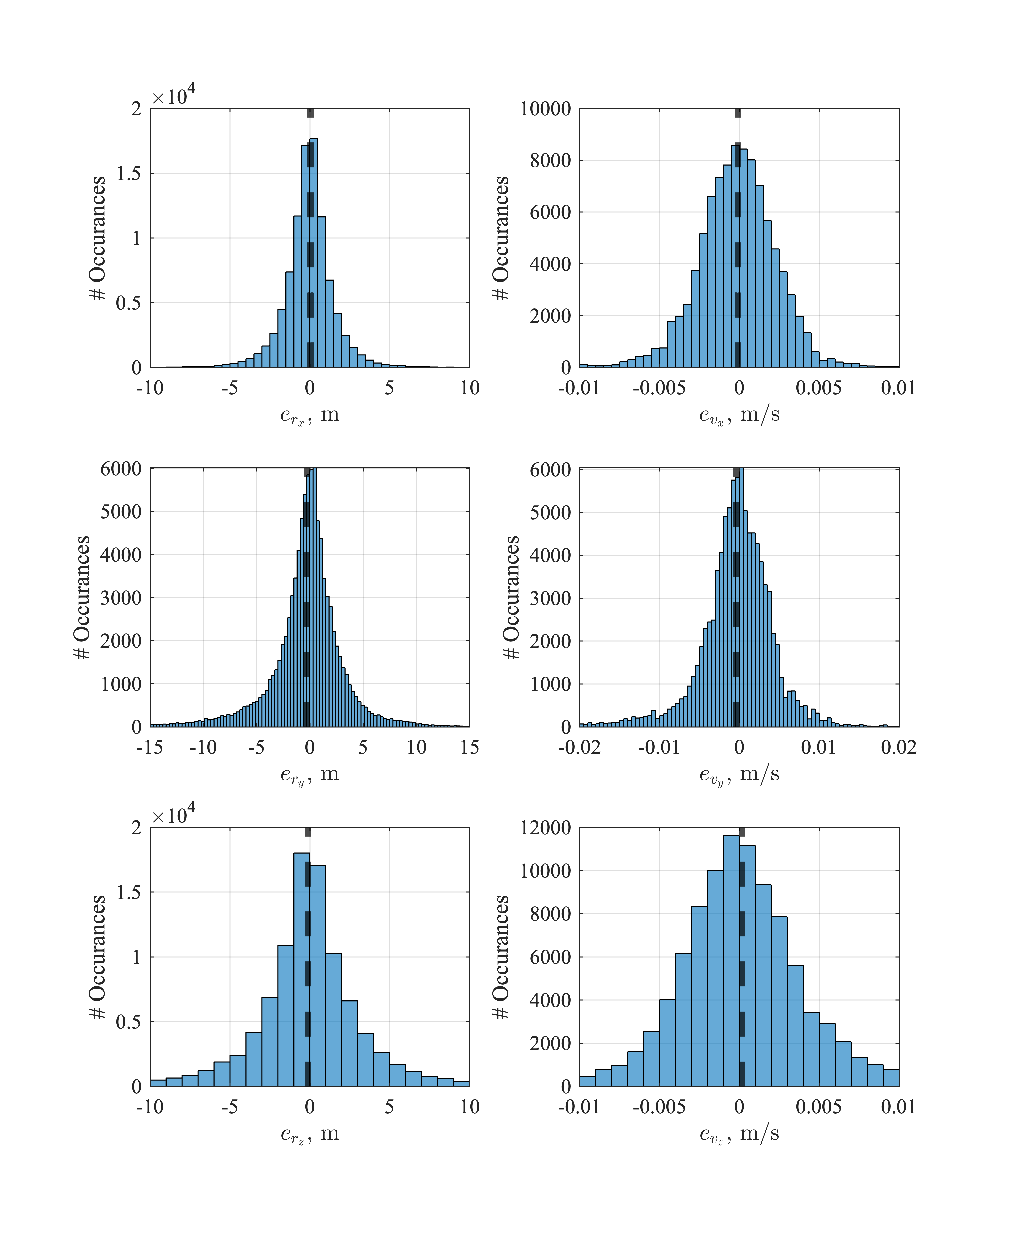
\includegraphics{./../../figures/UKFPosVelHist.eps}
	\caption{UKF Inertial State Estimation Error Distributions}
	\label{fig:UKFposvelhist}
\end{figure}

\begin{figure}
	\centering 
	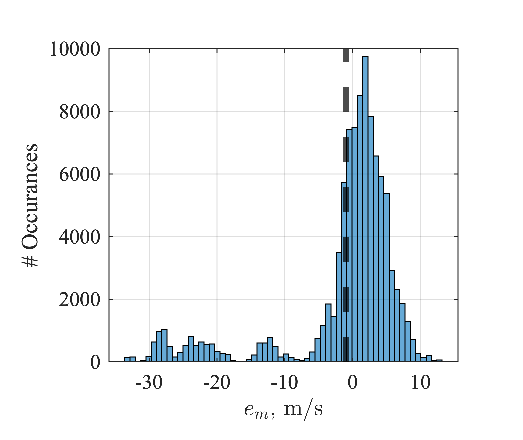
\includegraphics{./../../figures/UKFMassHist.eps}
	\caption{UKF Mass Estimation Error Distribution}
	\label{fig:UKFmasshist}
\end{figure}

As previously discussed for the EKF, to further investigate the distribution of the estimation errors and any bias present, Figures \ref{fig:UKFposvelhist} and \ref{fig:UKFmasshist} display histograms of the inertial states and mass respectively from each trial of the Monte Carlo analysis along with a vertical dashed line corresponding the mean of each distribution. 

Focusing first on the distributions of the inertial state estimation errors shown in Figure \ref{fig:EKFposvelhist}, we can see that a large majority of the errors again appear to be distributed normally with zero mean in all cases. Furthermore, the computed mean of each distribution is also near zero, quite different than observed for the EKF, and a highly desirable quality as bias in the estimated state can cause many problems with inertial navigation, especially if performing fully autonomous navigation and control of a spacecraft. Also, we can see the UKF was able to estimate the position of the spacecraft with much greater accuracy when compared to the EKF, with a majority occurrences falling within 10 m. Estimation accuracy of the velocity states did not see much improvement when compared to the EKF, although both filters did estimate the velocity of the spacecraft remarkably well. 

Shifting focus to Figure \ref{fig:UKFmasshist}, we see a similar trend as was observed for the EKF, with the distribution of mass estimation error appearing to exhibit multiple modes, although the mean of the distribution is near zero in this case. With that said, although the mean of the distribution is zero, each mode is centered far from zero, at around 3, -13, -25, and -29 kg. Furthermore, we can clearly observe that the UKF's ability to estimate the mass of the spacecraft is much worse than the EKF, with error growing as large as -35 kg in at least one of the trials performed. 

\section{Conclusions}
Overall, when comparing the performance of the EKF with the UKF at Earth GPS based inertial navigation in cislunar space, the UKF performed better, estimating the position of the spacecraft with much higher accuracy, all the while maintaining a better understanding of its estimation uncertainty and seemingly zero bias in estimation of all but the mass state. With that said, the UKF did perform very poor when estimating the mass of the spacecraft, and while the EKF did not estimate the mass with a high degree of accuracy, when compared to the UKF, it was much better. Both the EKF and UKF could likely be improved, either by incorporating a non-constant process noise as discussed in the preceding section, further tuning, or alternative strategies all together which would likely improve both filters ability to estimate the spacecrafts mass. 

Throughout this study, we've also found that use of the Earth based GPS constellation for inertial navigation in cislunar space is feasible and estimation accuracy of both the position and velocity of the spacecraft was achieved with high accuracy, especially when employing the UKF. It is important to note though that the trajectory used throughout this study was an ideal candidate for GPS based navigation, as the spacecraft was never eclipsed by the Moon. For the case of navigation of a spacecraft on the far side of the Moon or when traversing to the lunar surface, additional sensors or an additional GPS-like constellation of satellites in orbit about the Moon would very likely need to by employed.

\bibliographystyle{AAS_publication}   % Number the references.
\bibliography{references}   % Use references.bib to resolve the labels.

\end{document}
